\begin{frame}
    \begin{center}
        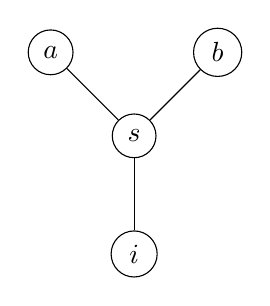
\begin{tikzpicture}[node distance={15mm},main/.style = {draw, circle}]
            \node[main] (s) {$s$};
            \node[main] (a) [above left of=s] {$a$};
            \node[main] (b) [above right of=s] {$b$};
            \node[main] (i) [below of=s] {$i$};
            \draw (s) -- (a);
            \draw (s) -- (b);
            \draw (s) -- (i);
        \end{tikzpicture}
    \end{center}
    Consider this network where we want to implement a firewall
    on the switch $s$.
    The goal of the firewall is to simply block all incoming packets.
    We define two events $a$ and $b$ representing the arrival of a packet
    on the switch from the hosts $a$ and $b$ respectively.
\end{frame}

\begin{frame}
    Assume that switch forwards all packets it received.
    We use an event $i$ to represent the forwarding of an arbitrary packet
    to $i$.
    So, we can represent this setting with an event structure $\mathrm{E}$
    with events $\s{a,b,i}$, an empty conflict relation and enabling relation
    the least one that satisfies:
    \begin{align*}
        \e \vdash a, \e \vdash b, \s{a} \vdash i, \s{b} \vdash i
    \end{align*}
\end{frame}

\begin{frame}
    The event structure of this network has the following configurations.
    Assume that $\sigma = \s{a,b,i}$ is given as a counterexample.
    We wish to find the cause of $\sigma \in \mathcal{F}(\mathrm{E})$.
    Assume that we want to declare $M(\s{a},i) = \T$ as a cause using
    the witness $(M(\s{b},i),\F,\F)$.
    \begin{center}
        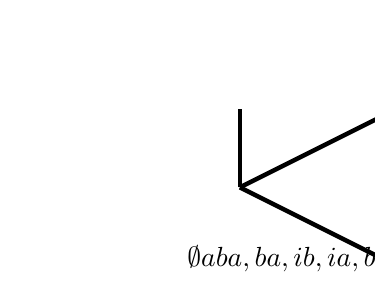
\begin{tikzpicture}
            \crd{0}{0}{$\emptyset$}
            \crd[left]{-2}{1}{$\s{a}$}
            \crd[right]{2}{1}{$\s{b}$}
            \crd[left]{0}{2}{$\s{a,b}$}
            \crd[above]{-2}{2}{$\s{a,i}$}
            \crd[above]{2}{2}{$\s{b,i}$}
            \crd[left]{0}{3}{$\s{a,b,i}$}
            \draw [ultra thick] (0,0) -- (-2,1);
            \draw [ultra thick] (0,0) -- (2,1);
            \draw [ultra thick] (-2,1) -- (0,2);
            \draw [ultra thick] (2,1) -- (0,2);
            \draw [ultra thick] (2,1) -- (2,2);
            \draw [ultra thick] (-2,1) -- (-2,2);
            \draw [ultra thick] (0,2) -- (0,3);
        \end{tikzpicture}
    \end{center}
\end{frame}

\begin{frame}
    \begin{center}
        \begin{tikzpicture}[node distance=20mm]
            \node [b] (eabi) {$EN(\s{a,b},i)$};
            \node [b] (ebi) [above left of=eabi] {$EN(\s{b},i)$};
            \node [b] (eai) [left of=ebi] {$EN(\s{a},i)$};
            \node [r] (eei) [above left of=ebi] {$EN(\e,i)$};
            \node [b] (mai) [above left of=eei] {$M(\s{a},i)$};
            \node [b] (mbi) [above right of=eei] {$M(\s{b},i)$};
            \node [r] (mei) [above left of=mbi] {$M(\e,i)$};
            \node [r] (mabi) [above of=mei,right of=mbi] {$M(\s{a,b},i)$};
            \node [r] (cab) [right of=mabi,below of=mabi] {$C(a,b)$};
            \draw [->] (mei) -- (mai);
            \draw [->] (mei) -- (mbi);
            \draw [->] (mai) -- (eai);
            \draw [->] (mei) -- (eei);
            \draw [->] (mbi) -- (ebi);
            \draw [->] (eei) -- (eai);
            \draw [->] (eei) -- (ebi);
            \draw [->] (mabi) -| (mai);
            \draw [->] (mabi) -- (mbi);
            \draw [->] (mabi) -- (eabi);
            \draw [->] (eai) -- (eabi);
            \draw [->] (ebi) -- (eabi);
            \draw [->] (cab) -- (eabi);
        \end{tikzpicture}
    \end{center}
\end{frame}

\begin{frame}
    \begin{center}
        \begin{tikzpicture}[node distance=20mm]
            \node [b] (eabi) {$EN(\s{a,b},i)$};
            \node [b] (ebi) [above left of=eabi] {$EN(\s{b},i)$};
            \node [b] (eai) [left of=ebi] {$EN(\s{a},i)$};
            \node [r] (eei) [above left of=ebi] {$EN(\e,i)$};
            \node [o] (mai) [above left of=eei] {$M(\s{a},i)$};
            \node [o] (mbi) [above right of=eei] {$M(\s{b},i)$};
            \node [r] (mei) [above left of=mbi] {$M(\e,i)$};
            \node [r] (mabi) [above of=mei,right of=mbi] {$M(\s{a,b},i)$};
            \node [r] (cab) [right of=mabi,below of=mabi] {$C(a,b)$};
            \draw [->] (mei) -- (mai);
            \draw [->] (mei) -- (mbi);
            \draw [->] (mai) -- (eai);
            \draw [->] (mei) -- (eei);
            \draw [->] (mbi) -- (ebi);
            \draw [->] (eei) -- (eai);
            \draw [->] (eei) -- (ebi);
            \draw [->] (mabi) -| (mai);
            \draw [->] (mabi) -- (mbi);
            \draw [->] (mabi) -- (eabi);
            \draw [->] (eai) -- (eabi);
            \draw [->] (ebi) -- (eabi);
            \draw [->] (cab) -- (eabi);
        \end{tikzpicture}
    \end{center}
\end{frame}

\begin{frame}
    \begin{center}
        \begin{tikzpicture}[node distance=20mm]
            \node [b] (eabi) {$EN(\s{a,b},i)$};
            \node [o] (ebi) [above left of=eabi] {$EN(\s{b},i)$};
            \node [o] (eai) [left of=ebi] {$EN(\s{a},i)$};
            \node [r] (eei) [above left of=ebi] {$EN(\e,i)$};
            \node [r] (mai) [above left of=eei] {$M(\s{a},i)$};
            \node [r] (mbi) [above right of=eei] {$M(\s{b},i)$};
            \node [r] (mei) [above left of=mbi] {$M(\e,i)$};
            \node [r] (mabi) [above of=mei,right of=mbi] {$M(\s{a,b},i)$};
            \node [r] (cab) [right of=mabi,below of=mabi] {$C(a,b)$};
            \draw [->] (mei) -- (mai);
            \draw [->] (mei) -- (mbi);
            \draw [->] (mai) -- (eai);
            \draw [->] (mei) -- (eei);
            \draw [->] (mbi) -- (ebi);
            \draw [->] (eei) -- (eai);
            \draw [->] (eei) -- (ebi);
            \draw [->] (mabi) -| (mai);
            \draw [->] (mabi) -- (mbi);
            \draw [->] (mabi) -- (eabi);
            \draw [->] (eai) -- (eabi);
            \draw [->] (ebi) -- (eabi);
            \draw [->] (cab) -- (eabi);
        \end{tikzpicture}
    \end{center}
\end{frame}

\begin{frame}
    \begin{center}
        \begin{tikzpicture}[node distance=20mm]
            \node [o] (eabi) {$EN(\s{a,b},i)$};
            \node [r] (ebi) [above left of=eabi] {$EN(\s{b},i)$};
            \node [r] (eai) [left of=ebi] {$EN(\s{a},i)$};
            \node [r] (eei) [above left of=ebi] {$EN(\e,i)$};
            \node [r] (mai) [above left of=eei] {$M(\s{a},i)$};
            \node [r] (mbi) [above right of=eei] {$M(\s{b},i)$};
            \node [r] (mei) [above left of=mbi] {$M(\e,i)$};
            \node [r] (mabi) [above of=mei,right of=mbi] {$M(\s{a,b},i)$};
            \node [r] (cab) [right of=mabi,below of=mabi] {$C(a,b)$};
            \draw [->] (mei) -- (mai);
            \draw [->] (mei) -- (mbi);
            \draw [->] (mai) -- (eai);
            \draw [->] (mei) -- (eei);
            \draw [->] (mbi) -- (ebi);
            \draw [->] (eei) -- (eai);
            \draw [->] (eei) -- (ebi);
            \draw [->] (mabi) -| (mai);
            \draw [->] (mabi) -- (mbi);
            \draw [->] (mabi) -- (eabi);
            \draw [->] (eai) -- (eabi);
            \draw [->] (ebi) -- (eabi);
            \draw [->] (cab) -- (eabi);
        \end{tikzpicture}
    \end{center}
\end{frame}

\begin{frame}
    \begin{center}
        \begin{tikzpicture}[node distance=20mm]
            \node [r] (eabi) {$EN(\s{a,b},i)$};
            \node [r] (ebi) [above left of=eabi] {$EN(\s{b},i)$};
            \node [r] (eai) [left of=ebi] {$EN(\s{a},i)$};
            \node [r] (eei) [above left of=ebi] {$EN(\e,i)$};
            \node [r] (mai) [above left of=eei] {$M(\s{a},i)$};
            \node [r] (mbi) [above right of=eei] {$M(\s{b},i)$};
            \node [r] (mei) [above left of=mbi] {$M(\e,i)$};
            \node [r] (mabi) [above of=mei,right of=mbi] {$M(\s{a,b},i)$};
            \node [r] (cab) [right of=mabi,below of=mabi] {$C(a,b)$};
            \draw [->] (mei) -- (mai);
            \draw [->] (mei) -- (mbi);
            \draw [->] (mai) -- (eai);
            \draw [->] (mei) -- (eei);
            \draw [->] (mbi) -- (ebi);
            \draw [->] (eei) -- (eai);
            \draw [->] (eei) -- (ebi);
            \draw [->] (mabi) -| (mai);
            \draw [->] (mabi) -- (mbi);
            \draw [->] (mabi) -- (eabi);
            \draw [->] (eai) -- (eabi);
            \draw [->] (ebi) -- (eabi);
            \draw [->] (cab) -- (eabi);
        \end{tikzpicture}
    \end{center}
\end{frame}

\begin{frame}
    \begin{align*}
        M & \vDash EN(\e,a)       = \T & \\
        M & \vDash EN(\s{b},a)    = \T & \\
        M & \vDash EN(\s{i},a)    = \T & \\
        M & \vDash EN(\s{b,i},a)  = \T & \\
        M & \vDash EN(\e,b)       = \T & \\
        M & \vDash EN(\s{a},b)    = \T & \\
        M & \vDash EN(\s{i},b)    = \T & \\
        M & \vDash EN(\s{a,i},b)  = \T & \\
        M & \vDash EN(\e,i)       = \F & \\
        M & \vDash EN(\s{a},i)    = \T & \\
        M & \vDash EN(\s{b},i)    = \T & \\
        M & \vDash EN(\s{a,b},i)  = \T & \\
    \end{align*}
\end{frame}

\begin{frame}
    \begin{align*}
        M & \vDash[M(\s{a},i)\la \F,M(\s{b},i)\la \F]EN(\e,a) = \T      & \\
        M & \vDash[M(\s{a},i)\la \F,M(\s{b},i)\la \F]EN(\s{b},a)= \T    & \\
        M & \vDash[M(\s{a},i)\la \F,M(\s{b},i)\la \F]EN(\s{i},a) = \T   & \\
        M & \vDash[M(\s{a},i)\la \F,M(\s{b},i)\la \F]EN(\s{b,i},a)= \T  & \\
        M & \vDash[M(\s{a},i)\la \F,M(\s{b},i)\la \F]EN(\e,b)   = \T    & \\
        M & \vDash[M(\s{a},i)\la \F,M(\s{b},i)\la \F]EN(\s{a},b) = \T   & \\
        M & \vDash[M(\s{a},i)\la \F,M(\s{b},i)\la \F]EN(\s{i},b) = \T   & \\
        M & \vDash[M(\s{a},i)\la \F,M(\s{b},i)\la \F]EN(\s{a,i},b) = \T & \\
        M & \vDash[M(\s{a},i)\la \F,M(\s{b},i)\la \F]EN(\e,i) = \F      & \\
        M & \vDash[M(\s{a},i)\la \F,M(\s{b},i)\la \F]EN(\s{a},i) = \F   & \\
        M & \vDash[M(\s{a},i)\la \F,M(\s{b},i)\la \F]EN(\s{b},i)  = \F  & \\
        M & \vDash[M(\s{a},i)\la \F,M(\s{b},i)\la \F]EN(\s{a,b},i)= \F  & \\
    \end{align*}
\end{frame}

\begin{frame}
    Thus, changing both $M(\s{a},i)$ and $M(\s{b},i)$ to false change
    configurations of the form in right:
    \begin{center}
        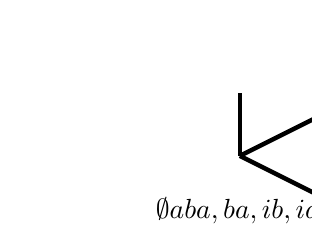
\begin{tikzpicture}[scale=0.8]
            \crd{0}{0}{$\emptyset$}
            \crd[left]{-2}{1}{$\s{a}$}
            \crd[right]{2}{1}{$\s{b}$}
            \crd[left]{0}{2}{$\s{a,b}$}
            \crd[above]{-2}{2}{$\s{a,i}$}
            \crd[above]{2}{2}{$\s{b,i}$}
            \crd[left]{0}{3}{$\s{a,b,i}$}
            \draw [ultra thick] (0,0) -- (-2,1);
            \draw [ultra thick] (0,0) -- (2,1);
            \draw [ultra thick] (-2,1) -- (0,2);
            \draw [ultra thick] (2,1) -- (0,2);
            \draw [ultra thick] (2,1) -- (2,2);
            \draw [ultra thick] (-2,1) -- (-2,2);
            \draw [ultra thick] (0,2) -- (0,3);
        \end{tikzpicture}
        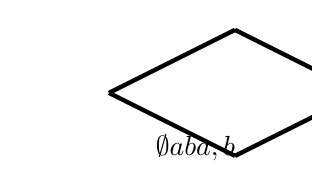
\begin{tikzpicture}[scale=0.8]
            \crd{0}{0}{$\emptyset$}
            \crd[left]{-2}{1}{$\s{a}$}
            \crd[right]{2}{1}{$\s{b}$}
            \crd[left]{0}{2}{$\s{a,b}$}
            \draw [ultra thick] (0,0) -- (-2,1);
            \draw [ultra thick] (0,0) -- (2,1);
            \draw [ultra thick] (-2,1) -- (0,2);
            \draw [ultra thick] (2,1) -- (0,2);
        \end{tikzpicture}
    \end{center}

\end{frame}

\begin{frame}
    Next, we need to check the AC2(b) condition:
    \begin{align*}
        M \vDash [M(\s{a},i)\la \T,M(\s{b},i) \la F, \vec Z' \la \vec z^*]
        \sigma \in \mathcal{\mathfrak{E}(\vec V)}
        \wedge \vec V = \vec v \wedge \vec v \in \mathcal{E}
    \end{align*}
    for all subsets $\vec Z'$ of $\vec Z$.
\end{frame}


\begin{frame}
    \begin{center}
        \begin{tikzpicture}[node distance=20mm]
            \node [b] (eabi) {$EN(\s{a,b},i)$};
            \node [b] (ebi) [above left of=eabi] {$EN(\s{b},i)$};
            \node [b] (eai) [left of=ebi] {$EN(\s{a},i)$};
            \node [r] (eei) [above left of=ebi] {$EN(\e,i)$};
            \node [b] (mai) [above left of=eei] {$M(\s{a},i)$};
            \node [b] (mbi) [above right of=eei] {$M(\s{b},i)$};
            \node [r] (mei) [above left of=mbi] {$M(\e,i)$};
            \node [r] (mabi) [above of=mei,right of=mbi] {$M(\s{a,b},i)$};
            \node [r] (cab) [right of=mabi,below of=mabi] {$C(a,b)$};
            \draw [->] (mei) -- (mai);
            \draw [->] (mei) -- (mbi);
            \draw [->] (mai) -- (eai);
            \draw [->] (mei) -- (eei);
            \draw [->] (mbi) -- (ebi);
            \draw [->] (eei) -- (eai);
            \draw [->] (eei) -- (ebi);
            \draw [->] (mabi) -| (mai);
            \draw [->] (mabi) -- (mbi);
            \draw [->] (mabi) -- (eabi);
            \draw [->] (eai) -- (eabi);
            \draw [->] (ebi) -- (eabi);
            \draw [->] (cab) -- (eabi);
        \end{tikzpicture}
    \end{center}
\end{frame}

\begin{frame}
    \begin{center}
        \begin{tikzpicture}[node distance=20mm]
            \node [b] (eabi) {$EN(\s{a,b},i)$};
            \node [b] (ebi) [above left of=eabi] {$EN(\s{b},i)$};
            \node [b] (eai) [left of=ebi] {$EN(\s{a},i)$};
            \node [r] (eei) [above left of=ebi] {$EN(\e,i)$};
            \node [o] (mai) [above left of=eei] {$M(\s{a},i)$};
            \node [o] (mbi) [above right of=eei] {$M(\s{b},i)$};
            \node [r] (mei) [above left of=mbi] {$M(\e,i)$};
            \node [r] (mabi) [above of=mei,right of=mbi] {$M(\s{a,b},i)$};
            \node [r] (cab) [right of=mabi,below of=mabi] {$C(a,b)$};
            \draw [->] (mei) -- (mai);
            \draw [->] (mei) -- (mbi);
            \draw [->] (mai) -- (eai);
            \draw [->] (mei) -- (eei);
            \draw [->] (mbi) -- (ebi);
            \draw [->] (eei) -- (eai);
            \draw [->] (eei) -- (ebi);
            \draw [->] (mabi) -| (mai);
            \draw [->] (mabi) -- (mbi);
            \draw [->] (mabi) -- (eabi);
            \draw [->] (eai) -- (eabi);
            \draw [->] (ebi) -- (eabi);
            \draw [->] (cab) -- (eabi);
        \end{tikzpicture}
    \end{center}
\end{frame}

\begin{frame}
    \begin{center}
        \begin{tikzpicture}[node distance=20mm]
            \node [b] (eabi) {$EN(\s{a,b},i)$};
            \node [o] (ebi) [above left of=eabi] {$EN(\s{b},i)$};
            \node [o] (eai) [left of=ebi] {$EN(\s{a},i)$};
            \node [r] (eei) [above left of=ebi] {$EN(\e,i)$};
            \node [b] (mai) [above left of=eei] {$M(\s{a},i)$};
            \node [r] (mbi) [above right of=eei] {$M(\s{b},i)$};
            \node [r] (mei) [above left of=mbi] {$M(\e,i)$};
            \node [r] (mabi) [above of=mei,right of=mbi] {$M(\s{a,b},i)$};
            \node [r] (cab) [right of=mabi,below of=mabi] {$C(a,b)$};
            \draw [->] (mei) -- (mai);
            \draw [->] (mei) -- (mbi);
            \draw [->] (mai) -- (eai);
            \draw [->] (mei) -- (eei);
            \draw [->] (mbi) -- (ebi);
            \draw [->] (eei) -- (eai);
            \draw [->] (eei) -- (ebi);
            \draw [->] (mabi) -| (mai);
            \draw [->] (mabi) -- (mbi);
            \draw [->] (mabi) -- (eabi);
            \draw [->] (eai) -- (eabi);
            \draw [->] (ebi) -- (eabi);
            \draw [->] (cab) -- (eabi);
        \end{tikzpicture}
    \end{center}
\end{frame}

\begin{frame}
    \begin{center}
        \begin{tikzpicture}[node distance=20mm]
            \node [o] (eabi) {$EN(\s{a,b},i)$};
            \node [r] (ebi) [above left of=eabi] {$EN(\s{b},i)$};
            \node [b] (eai) [left of=ebi] {$EN(\s{a},i)$};
            \node [r] (eei) [above left of=ebi] {$EN(\e,i)$};
            \node [b] (mai) [above left of=eei] {$M(\s{a},i)$};
            \node [r] (mbi) [above right of=eei] {$M(\s{b},i)$};
            \node [r] (mei) [above left of=mbi] {$M(\e,i)$};
            \node [r] (mabi) [above of=mei,right of=mbi] {$M(\s{a,b},i)$};
            \node [r] (cab) [right of=mabi,below of=mabi] {$C(a,b)$};
            \draw [->] (mei) -- (mai);
            \draw [->] (mei) -- (mbi);
            \draw [->] (mai) -- (eai);
            \draw [->] (mei) -- (eei);
            \draw [->] (mbi) -- (ebi);
            \draw [->] (eei) -- (eai);
            \draw [->] (eei) -- (ebi);
            \draw [->] (mabi) -| (mai);
            \draw [->] (mabi) -- (mbi);
            \draw [->] (mabi) -- (eabi);
            \draw [->] (eai) -- (eabi);
            \draw [->] (ebi) -- (eabi);
            \draw [->] (cab) -- (eabi);
        \end{tikzpicture}
    \end{center}
\end{frame}

\begin{frame}
    \begin{center}
        \begin{tikzpicture}[node distance=20mm]
            \node [b] (eabi) {$EN(\s{a,b},i)$};
            \node [r] (ebi) [above left of=eabi] {$EN(\s{b},i)$};
            \node [b] (eai) [left of=ebi] {$EN(\s{a},i)$};
            \node [r] (eei) [above left of=ebi] {$EN(\e,i)$};
            \node [b] (mai) [above left of=eei] {$M(\s{a},i)$};
            \node [r] (mbi) [above right of=eei] {$M(\s{b},i)$};
            \node [r] (mei) [above left of=mbi] {$M(\e,i)$};
            \node [r] (mabi) [above of=mei,right of=mbi] {$M(\s{a,b},i)$};
            \node [r] (cab) [right of=mabi,below of=mabi] {$C(a,b)$};
            \draw [->] (mei) -- (mai);
            \draw [->] (mei) -- (mbi);
            \draw [->] (mai) -- (eai);
            \draw [->] (mei) -- (eei);
            \draw [->] (mbi) -- (ebi);
            \draw [->] (eei) -- (eai);
            \draw [->] (eei) -- (ebi);
            \draw [->] (mabi) -| (mai);
            \draw [->] (mabi) -- (mbi);
            \draw [->] (mabi) -- (eabi);
            \draw [->] (eai) -- (eabi);
            \draw [->] (ebi) -- (eabi);
            \draw [->] (cab) -- (eabi);
        \end{tikzpicture}
    \end{center}
\end{frame}

\begin{frame}
    We can conclude that by setting $M(\s{b},i)$ to false only
    $EN(\s{b},i)$ and $M(\s{b},i)$ itself change their value.
    Thus, we only need to verify the following cases:
    \begin{align*}
        M & \vDash[M(\s{a},i)\la \T,M(\s{b},i)\la \F] & \sigma \in \mathcal{\mathfrak{E}(\vec V)}
        \wedge \vec V = \vec v \wedge \vec v \in \mathcal{E} \\
        M & \vDash[M(\s{a},i)\la \T,M(\s{b},i)\la \F,EN(\s{b},i)\la T] &\sigma \in \mathcal{\mathfrak{E}(\vec V)}
        \wedge \vec V = \vec v \wedge \vec v \in \mathcal{E}
    \end{align*}
\end{frame}